\documentclass[twoside]{book}

% Packages required by doxygen
\usepackage{fixltx2e}
\usepackage{calc}
\usepackage{doxygen}
\usepackage[export]{adjustbox} % also loads graphicx
\usepackage{graphicx}
\usepackage[utf8]{inputenc}
\usepackage{makeidx}
\usepackage{multicol}
\usepackage{multirow}
\PassOptionsToPackage{warn}{textcomp}
\usepackage{textcomp}
\usepackage[nointegrals]{wasysym}
\usepackage[table]{xcolor}

% Font selection
\usepackage[T1]{fontenc}
\usepackage[scaled=.90]{helvet}
\usepackage{courier}
\usepackage{amssymb}
\usepackage{sectsty}
\renewcommand{\familydefault}{\sfdefault}
\allsectionsfont{%
  \fontseries{bc}\selectfont%
  \color{darkgray}%
}
\renewcommand{\DoxyLabelFont}{%
  \fontseries{bc}\selectfont%
  \color{darkgray}%
}
\newcommand{\+}{\discretionary{\mbox{\scriptsize$\hookleftarrow$}}{}{}}

% Page & text layout
\usepackage{geometry}
\geometry{%
  a4paper,%
  top=2.5cm,%
  bottom=2.5cm,%
  left=2.5cm,%
  right=2.5cm%
}
\tolerance=750
\hfuzz=15pt
\hbadness=750
\setlength{\emergencystretch}{15pt}
\setlength{\parindent}{0cm}
\setlength{\parskip}{3ex plus 2ex minus 2ex}
\makeatletter
\renewcommand{\paragraph}{%
  \@startsection{paragraph}{4}{0ex}{-1.0ex}{1.0ex}{%
    \normalfont\normalsize\bfseries\SS@parafont%
  }%
}
\renewcommand{\subparagraph}{%
  \@startsection{subparagraph}{5}{0ex}{-1.0ex}{1.0ex}{%
    \normalfont\normalsize\bfseries\SS@subparafont%
  }%
}
\makeatother

% Headers & footers
\usepackage{fancyhdr}
\pagestyle{fancyplain}
\fancyhead[LE]{\fancyplain{}{\bfseries\thepage}}
\fancyhead[CE]{\fancyplain{}{}}
\fancyhead[RE]{\fancyplain{}{\bfseries\leftmark}}
\fancyhead[LO]{\fancyplain{}{\bfseries\rightmark}}
\fancyhead[CO]{\fancyplain{}{}}
\fancyhead[RO]{\fancyplain{}{\bfseries\thepage}}
\fancyfoot[LE]{\fancyplain{}{}}
\fancyfoot[CE]{\fancyplain{}{}}
\fancyfoot[RE]{\fancyplain{}{\bfseries\scriptsize Generated by Doxygen }}
\fancyfoot[LO]{\fancyplain{}{\bfseries\scriptsize Generated by Doxygen }}
\fancyfoot[CO]{\fancyplain{}{}}
\fancyfoot[RO]{\fancyplain{}{}}
\renewcommand{\footrulewidth}{0.4pt}
\renewcommand{\chaptermark}[1]{%
  \markboth{#1}{}%
}
\renewcommand{\sectionmark}[1]{%
  \markright{\thesection\ #1}%
}

% Indices & bibliography
\usepackage{natbib}
\usepackage[titles]{tocloft}
\setcounter{tocdepth}{3}
\setcounter{secnumdepth}{5}
\makeindex

% Hyperlinks (required, but should be loaded last)
\usepackage{ifpdf}
\ifpdf
  \usepackage[pdftex,pagebackref=true]{hyperref}
\else
  \usepackage[ps2pdf,pagebackref=true]{hyperref}
\fi
\hypersetup{%
  colorlinks=true,%
  linkcolor=blue,%
  citecolor=blue,%
  unicode%
}

% Custom commands
\newcommand{\clearemptydoublepage}{%
  \newpage{\pagestyle{empty}\cleardoublepage}%
}

\usepackage{caption}
\captionsetup{labelsep=space,justification=centering,font={bf},singlelinecheck=off,skip=4pt,position=top}

%===== C O N T E N T S =====

\begin{document}

% Titlepage & ToC
\hypersetup{pageanchor=false,
             bookmarksnumbered=true,
             pdfencoding=unicode
            }
\pagenumbering{alph}
\begin{titlepage}
\vspace*{7cm}
\begin{center}%
{\Large Match Game \\[1ex]\large 1a }\\
\vspace*{1cm}
{\large Generated by Doxygen 1.8.13}\\
\end{center}
\end{titlepage}
\clearemptydoublepage
\pagenumbering{roman}
\tableofcontents
\clearemptydoublepage
\pagenumbering{arabic}
\hypersetup{pageanchor=true}

%--- Begin generated contents ---
\chapter{Hierarchical Index}
\section{Class Hierarchy}
This inheritance list is sorted roughly, but not completely, alphabetically\+:\begin{DoxyCompactList}
\item Mono\+Behaviour\begin{DoxyCompactList}
\item \contentsline{section}{Circular\+Element}{\pageref{class_circular_element}}{}
\item \contentsline{section}{Color\+Pallete}{\pageref{class_color_pallete}}{}
\item \contentsline{section}{Command\+Button}{\pageref{class_command_button}}{}
\item \contentsline{section}{Game\+Manager}{\pageref{class_game_manager}}{}
\item \contentsline{section}{Grid}{\pageref{class_grid}}{}
\item \contentsline{section}{Menu\+Script}{\pageref{class_menu_script}}{}
\item \contentsline{section}{Random\+Color}{\pageref{class_random_color}}{}
\item \contentsline{section}{Tutorial\+Script}{\pageref{class_tutorial_script}}{}
\end{DoxyCompactList}
\item \contentsline{section}{Pallete}{\pageref{struct_pallete}}{}
\item Scriptable\+Object\begin{DoxyCompactList}
\item \contentsline{section}{Color\+Transition}{\pageref{class_color_transition}}{}
\end{DoxyCompactList}
\end{DoxyCompactList}

\chapter{Class Index}
\section{Class List}
Here are the classes, structs, unions and interfaces with brief descriptions\+:\begin{DoxyCompactList}
\item\contentsline{section}{\hyperlink{class_circular_element}{Circular\+Element} }{\pageref{class_circular_element}}{}
\item\contentsline{section}{\hyperlink{class_color_pallete}{Color\+Pallete} }{\pageref{class_color_pallete}}{}
\item\contentsline{section}{\hyperlink{class_color_transition}{Color\+Transition} }{\pageref{class_color_transition}}{}
\item\contentsline{section}{\hyperlink{class_command_button}{Command\+Button} }{\pageref{class_command_button}}{}
\item\contentsline{section}{\hyperlink{class_game_manager}{Game\+Manager} }{\pageref{class_game_manager}}{}
\item\contentsline{section}{\hyperlink{class_grid}{Grid} }{\pageref{class_grid}}{}
\item\contentsline{section}{\hyperlink{class_menu_script}{Menu\+Script} }{\pageref{class_menu_script}}{}
\item\contentsline{section}{\hyperlink{struct_pallete}{Pallete} }{\pageref{struct_pallete}}{}
\item\contentsline{section}{\hyperlink{class_random_color}{Random\+Color} }{\pageref{class_random_color}}{}
\item\contentsline{section}{\hyperlink{class_tutorial_script}{Tutorial\+Script} }{\pageref{class_tutorial_script}}{}
\end{DoxyCompactList}

\chapter{Class Documentation}
\hypertarget{class_circular_element}{}\section{Circular\+Element Class Reference}
\label{class_circular_element}\index{Circular\+Element@{Circular\+Element}}
Inheritance diagram for Circular\+Element\+:\begin{figure}[H]
\begin{center}
\leavevmode
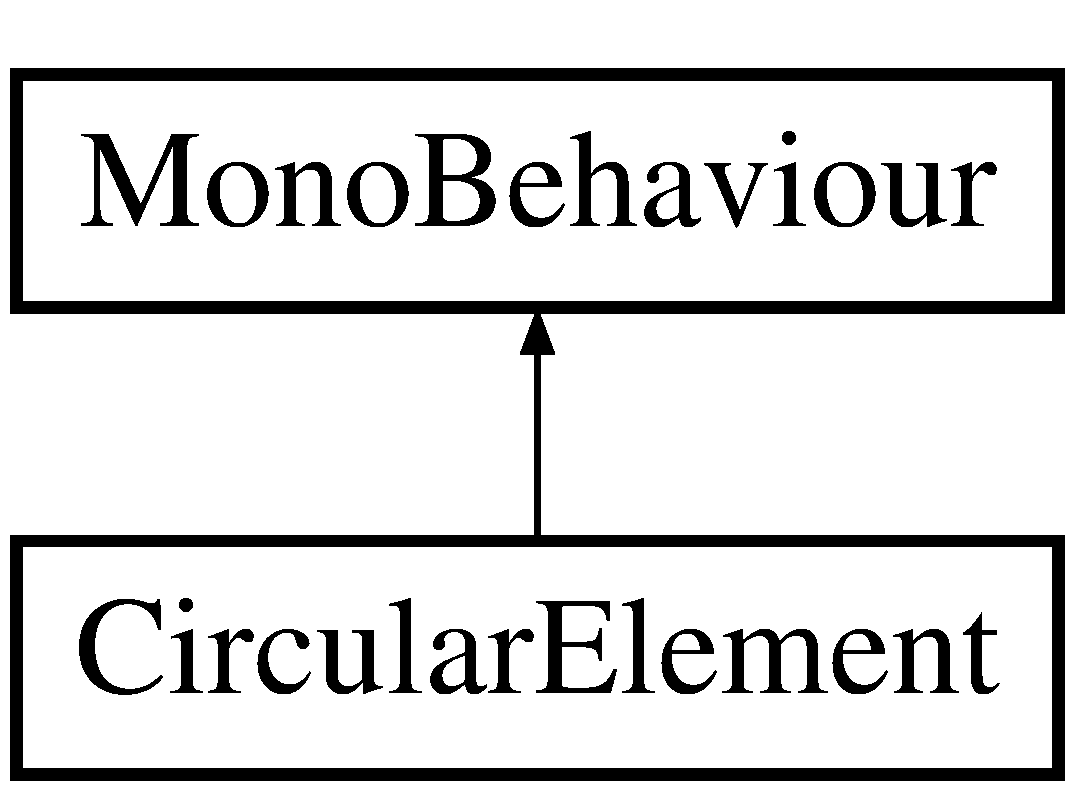
\includegraphics[height=2.000000cm]{class_circular_element}
\end{center}
\end{figure}
\subsection*{Public Member Functions}
\begin{DoxyCompactItemize}
\item 
\mbox{\Hypertarget{class_circular_element_ae7c9c04c0e02283602c34a7bf0a5c1b0}\label{class_circular_element_ae7c9c04c0e02283602c34a7bf0a5c1b0}} 
Mesh {\bfseries Make\+Circle} (int num\+Of\+Points)
\item 
\mbox{\Hypertarget{class_circular_element_a4eb5a7f5890b2ce9c26f2b83d8390320}\label{class_circular_element_a4eb5a7f5890b2ce9c26f2b83d8390320}} 
void {\bfseries Set\+Material} (Material material)
\end{DoxyCompactItemize}
\subsection*{Public Attributes}
\begin{DoxyCompactItemize}
\item 
\mbox{\Hypertarget{class_circular_element_a4d50d6f56387cb2ab0e49997d04459a5}\label{class_circular_element_a4d50d6f56387cb2ab0e49997d04459a5}} 
float {\bfseries circular\+Radius} = 0.\+5f
\item 
float \hyperlink{class_circular_element_a9442a4ccbffb0581a724e1fb1cdea53f}{angle\+Size} = 360f
\item 
\mbox{\Hypertarget{class_circular_element_a7a4d50b83e1c51cab0667d6c2bd7b713}\label{class_circular_element_a7a4d50b83e1c51cab0667d6c2bd7b713}} 
int {\bfseries num\+Of\+Points}
\item 
\mbox{\Hypertarget{class_circular_element_ae823fbe8cf80972c9ccefb02b8f36cf6}\label{class_circular_element_ae823fbe8cf80972c9ccefb02b8f36cf6}} 
Shader {\bfseries my\+Shader}
\end{DoxyCompactItemize}


\subsection{Member Data Documentation}
\mbox{\Hypertarget{class_circular_element_a9442a4ccbffb0581a724e1fb1cdea53f}\label{class_circular_element_a9442a4ccbffb0581a724e1fb1cdea53f}} 
\index{Circular\+Element@{Circular\+Element}!angle\+Size@{angle\+Size}}
\index{angle\+Size@{angle\+Size}!Circular\+Element@{Circular\+Element}}
\subsubsection{\texorpdfstring{angle\+Size}{angleSize}}
{\footnotesize\ttfamily float Circular\+Element.\+angle\+Size = 360f}

$<$ Angulo do mesh a ser gerado 

The documentation for this class was generated from the following file\+:\begin{DoxyCompactItemize}
\item 
Circular\+Element.\+cs\end{DoxyCompactItemize}

\hypertarget{class_color_pallete}{}\section{Color\+Pallete Class Reference}
\label{class_color_pallete}\index{Color\+Pallete@{Color\+Pallete}}
Inheritance diagram for Color\+Pallete\+:\begin{figure}[H]
\begin{center}
\leavevmode
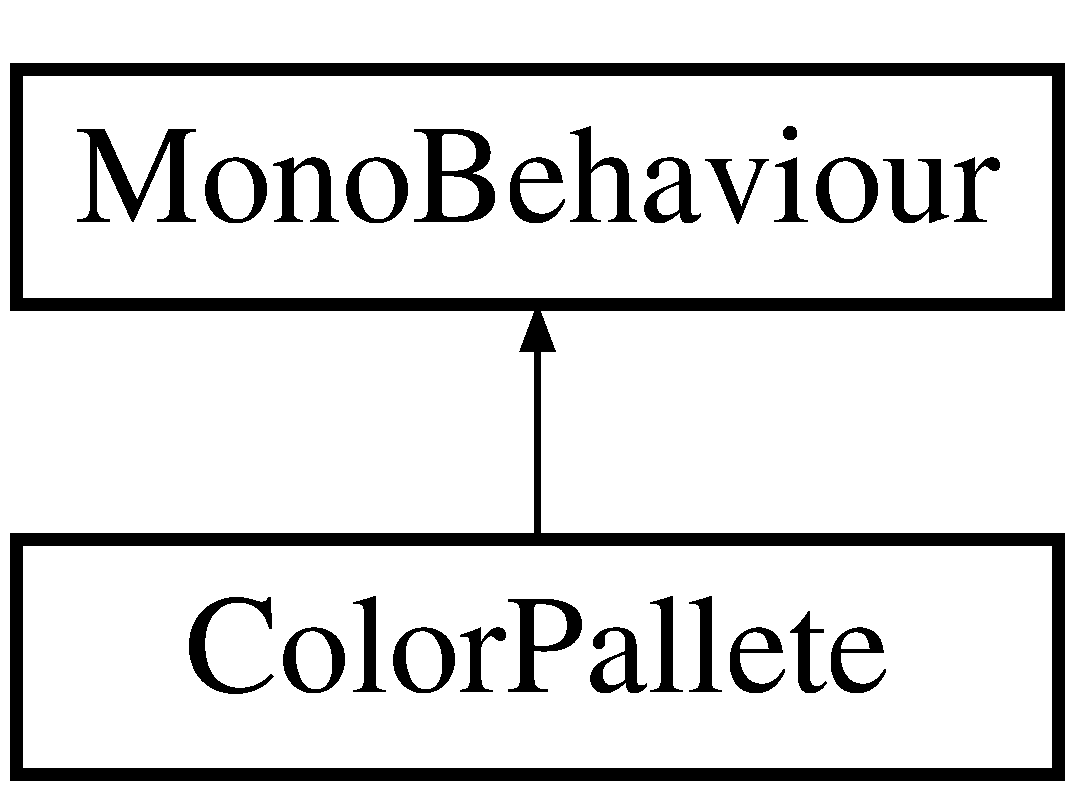
\includegraphics[height=2.000000cm]{class_color_pallete}
\end{center}
\end{figure}


The documentation for this class was generated from the following file\+:\begin{DoxyCompactItemize}
\item 
Color\+Pallete.\+cs\end{DoxyCompactItemize}

\hypertarget{class_color_transition}{}\section{Color\+Transition Class Reference}
\label{class_color_transition}\index{Color\+Transition@{Color\+Transition}}
Inheritance diagram for Color\+Transition\+:\begin{figure}[H]
\begin{center}
\leavevmode
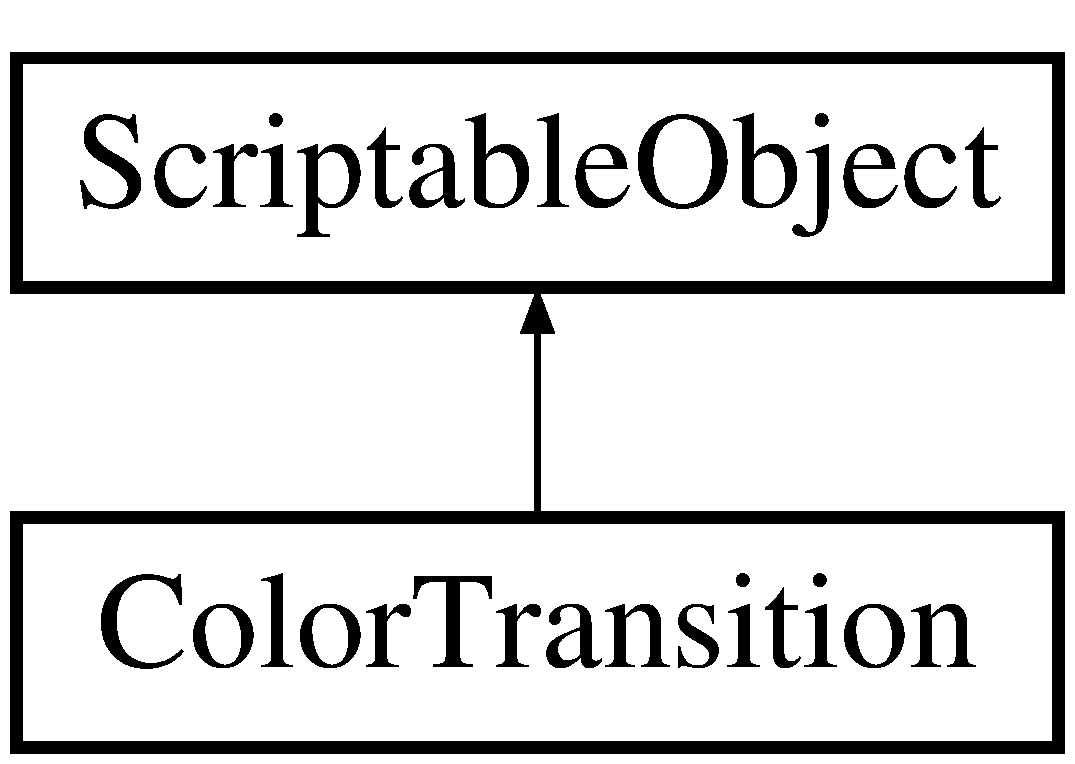
\includegraphics[height=2.000000cm]{class_color_transition}
\end{center}
\end{figure}
\subsection*{Public Member Functions}
\begin{DoxyCompactItemize}
\item 
\mbox{\Hypertarget{class_color_transition_a6847c2bd73b2e3ba61d7b40b9bdfcece}\label{class_color_transition_a6847c2bd73b2e3ba61d7b40b9bdfcece}} 
I\+Enumerator {\bfseries Swap\+Color} (Material \+\_\+mat, Color B)
\end{DoxyCompactItemize}
\subsection*{Public Attributes}
\begin{DoxyCompactItemize}
\item 
\mbox{\Hypertarget{class_color_transition_a9e087042afcc0f0b15a34e6e169929ca}\label{class_color_transition_a9e087042afcc0f0b15a34e6e169929ca}} 
Color {\bfseries ColorB}
\item 
\mbox{\Hypertarget{class_color_transition_a0e62c2c0867491712081253f77e2cc4e}\label{class_color_transition_a0e62c2c0867491712081253f77e2cc4e}} 
Material {\bfseries mat}
\item 
\mbox{\Hypertarget{class_color_transition_a23b872d57138292d6b6080e80ac437bf}\label{class_color_transition_a23b872d57138292d6b6080e80ac437bf}} 
float {\bfseries swap\+Value}
\item 
\mbox{\Hypertarget{class_color_transition_ac163cb483b00da7ea1b54c26e07c1fee}\label{class_color_transition_ac163cb483b00da7ea1b54c26e07c1fee}} 
float {\bfseries duration}
\end{DoxyCompactItemize}


The documentation for this class was generated from the following file\+:\begin{DoxyCompactItemize}
\item 
Color\+Transition.\+cs\end{DoxyCompactItemize}

\hypertarget{class_command_button}{}\section{Command\+Button Class Reference}
\label{class_command_button}\index{Command\+Button@{Command\+Button}}
Inheritance diagram for Command\+Button\+:\begin{figure}[H]
\begin{center}
\leavevmode
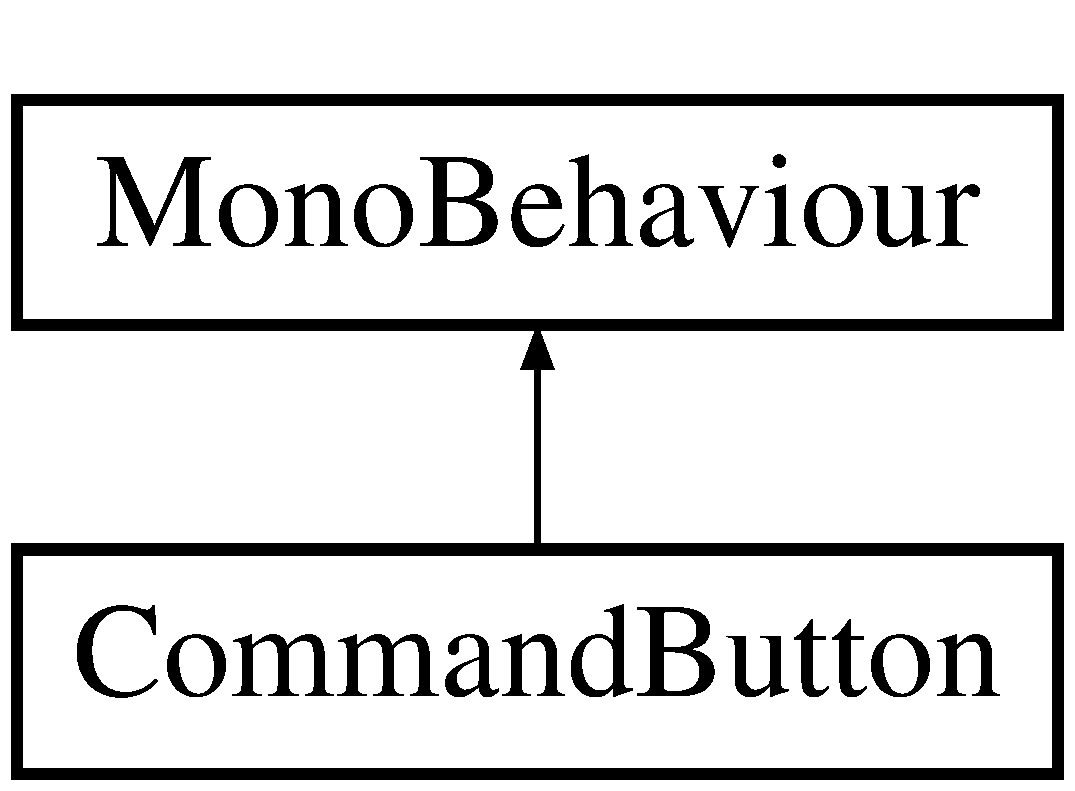
\includegraphics[height=2.000000cm]{class_command_button}
\end{center}
\end{figure}
\subsection*{Public Member Functions}
\begin{DoxyCompactItemize}
\item 
\mbox{\Hypertarget{class_command_button_a76a4cf105f8225511db815cbda5d93fe}\label{class_command_button_a76a4cf105f8225511db815cbda5d93fe}} 
void {\bfseries Button\+Command} (Vector2 Pos\+World2D)
\end{DoxyCompactItemize}


The documentation for this class was generated from the following file\+:\begin{DoxyCompactItemize}
\item 
Command\+Button.\+cs\end{DoxyCompactItemize}

\hypertarget{class_game_manager}{}\section{Game\+Manager Class Reference}
\label{class_game_manager}\index{Game\+Manager@{Game\+Manager}}
Inheritance diagram for Game\+Manager\+:\begin{figure}[H]
\begin{center}
\leavevmode
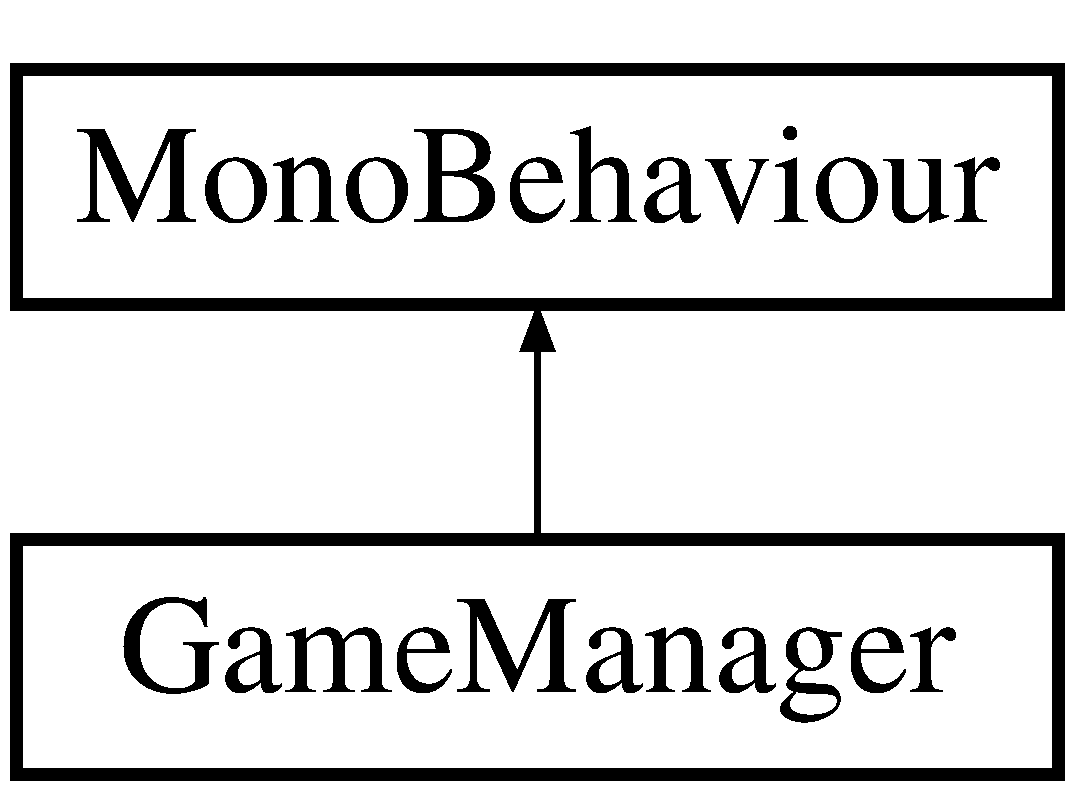
\includegraphics[height=2.000000cm]{class_game_manager}
\end{center}
\end{figure}
\subsection*{Public Member Functions}
\begin{DoxyCompactItemize}
\item 
\mbox{\Hypertarget{class_game_manager_a9ca299160f5af64bf3b19da2d2fa0feb}\label{class_game_manager_a9ca299160f5af64bf3b19da2d2fa0feb}} 
void {\bfseries Load\+Object} (Transform touch\+Object)
\end{DoxyCompactItemize}
\subsection*{Public Attributes}
\begin{DoxyCompactItemize}
\item 
\mbox{\Hypertarget{class_game_manager_a5d670dd9d695d7401b98017fe483cdd9}\label{class_game_manager_a5d670dd9d695d7401b98017fe483cdd9}} 
List$<$ Transform $>$ {\bfseries touch\+Objects}
\item 
\mbox{\Hypertarget{class_game_manager_a564b08c23d0ca3bac1e81786e8b37ca9}\label{class_game_manager_a564b08c23d0ca3bac1e81786e8b37ca9}} 
float {\bfseries time\+Taken\+During\+Lerp} = 1f
\end{DoxyCompactItemize}
\subsection*{Properties}
\begin{DoxyCompactItemize}
\item 
\mbox{\Hypertarget{class_game_manager_ad3e717f4fb0f378b969f4457de81f23e}\label{class_game_manager_ad3e717f4fb0f378b969f4457de81f23e}} 
static \hyperlink{class_game_manager}{Game\+Manager} {\bfseries Instance}\hspace{0.3cm}{\ttfamily  \mbox{[}get\mbox{]}}
\end{DoxyCompactItemize}


The documentation for this class was generated from the following file\+:\begin{DoxyCompactItemize}
\item 
Game\+Manager.\+cs\end{DoxyCompactItemize}

\hypertarget{class_grid}{}\section{Grid Class Reference}
\label{class_grid}\index{Grid@{Grid}}
Inheritance diagram for Grid\+:\begin{figure}[H]
\begin{center}
\leavevmode
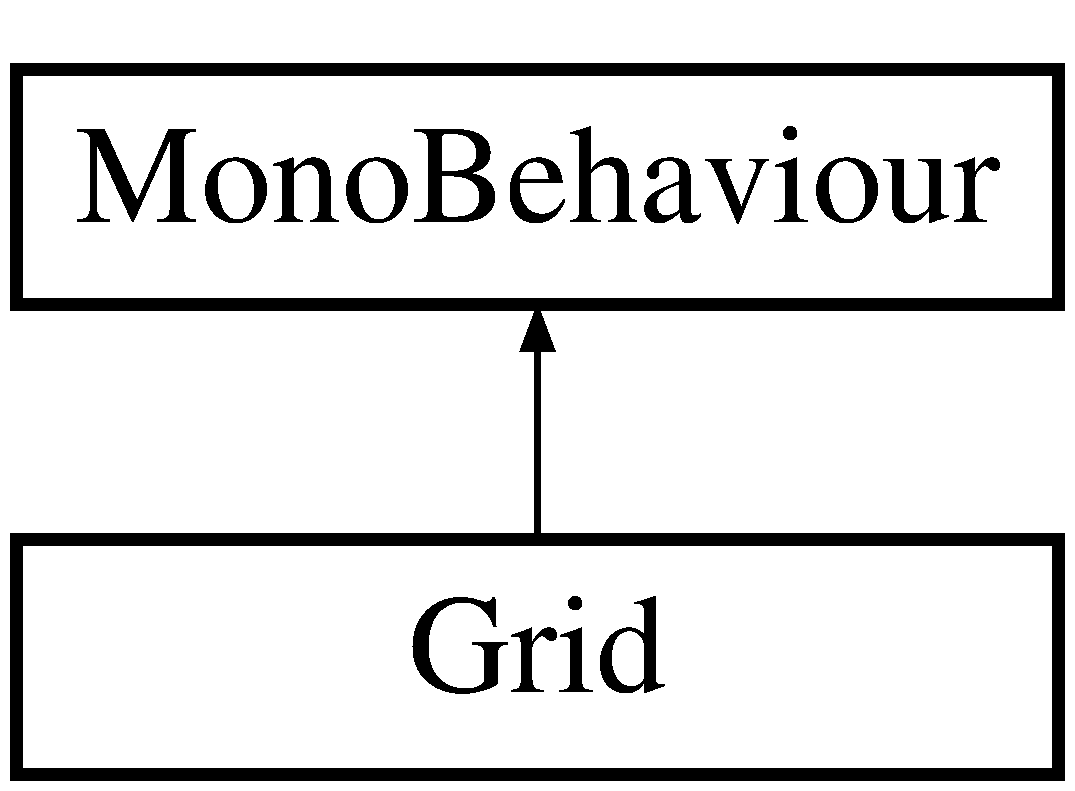
\includegraphics[height=2.000000cm]{class_grid}
\end{center}
\end{figure}
\subsection*{Public Member Functions}
\begin{DoxyCompactItemize}
\item 
\mbox{\Hypertarget{class_grid_ac21bfc827b59e29af93cf38cfeef71b7}\label{class_grid_ac21bfc827b59e29af93cf38cfeef71b7}} 
void {\bfseries Clean\+Grid} ()
\item 
\mbox{\Hypertarget{class_grid_a8ae55ecdb63003b0e0b225bf057c7703}\label{class_grid_a8ae55ecdb63003b0e0b225bf057c7703}} 
void {\bfseries Generate\+Grid} (int x\+Size, int y\+Size)
\item 
\mbox{\Hypertarget{class_grid_aa5bae6cb91c6d9fd4e01b28c27281bce}\label{class_grid_aa5bae6cb91c6d9fd4e01b28c27281bce}} 
I\+Enumerator {\bfseries Generate\+Elements} ()
\item 
\mbox{\Hypertarget{class_grid_ad94667c037068a4fcb29523d04079ac8}\label{class_grid_ad94667c037068a4fcb29523d04079ac8}} 
void {\bfseries Generate} ()
\end{DoxyCompactItemize}
\subsection*{Public Attributes}
\begin{DoxyCompactItemize}
\item 
\mbox{\Hypertarget{class_grid_a58b61c766bade49f79f34e0077ea05b6}\label{class_grid_a58b61c766bade49f79f34e0077ea05b6}} 
int {\bfseries x\+Size}
\item 
\mbox{\Hypertarget{class_grid_a9937b5b55c3dbe77aa73edcac15f04bf}\label{class_grid_a9937b5b55c3dbe77aa73edcac15f04bf}} 
\hyperlink{class_circular_element}{Circular\+Element} {\bfseries circle\+Ref}
\item 
\mbox{\Hypertarget{class_grid_ad1c6c49c18d89e95946edbf84eddd73c}\label{class_grid_ad1c6c49c18d89e95946edbf84eddd73c}} 
float {\bfseries min\+Distance}
\end{DoxyCompactItemize}
\subsection*{Properties}
\begin{DoxyCompactItemize}
\item 
\mbox{\Hypertarget{class_grid_ad1f5343530730e0088210d636be646ed}\label{class_grid_ad1f5343530730e0088210d636be646ed}} 
static \hyperlink{class_grid}{Grid} {\bfseries Instance}\hspace{0.3cm}{\ttfamily  \mbox{[}get\mbox{]}}
\end{DoxyCompactItemize}


The documentation for this class was generated from the following file\+:\begin{DoxyCompactItemize}
\item 
Grid.\+cs\end{DoxyCompactItemize}

\hypertarget{class_menu_script}{}\section{Menu\+Script Class Reference}
\label{class_menu_script}\index{Menu\+Script@{Menu\+Script}}
Inheritance diagram for Menu\+Script\+:\begin{figure}[H]
\begin{center}
\leavevmode
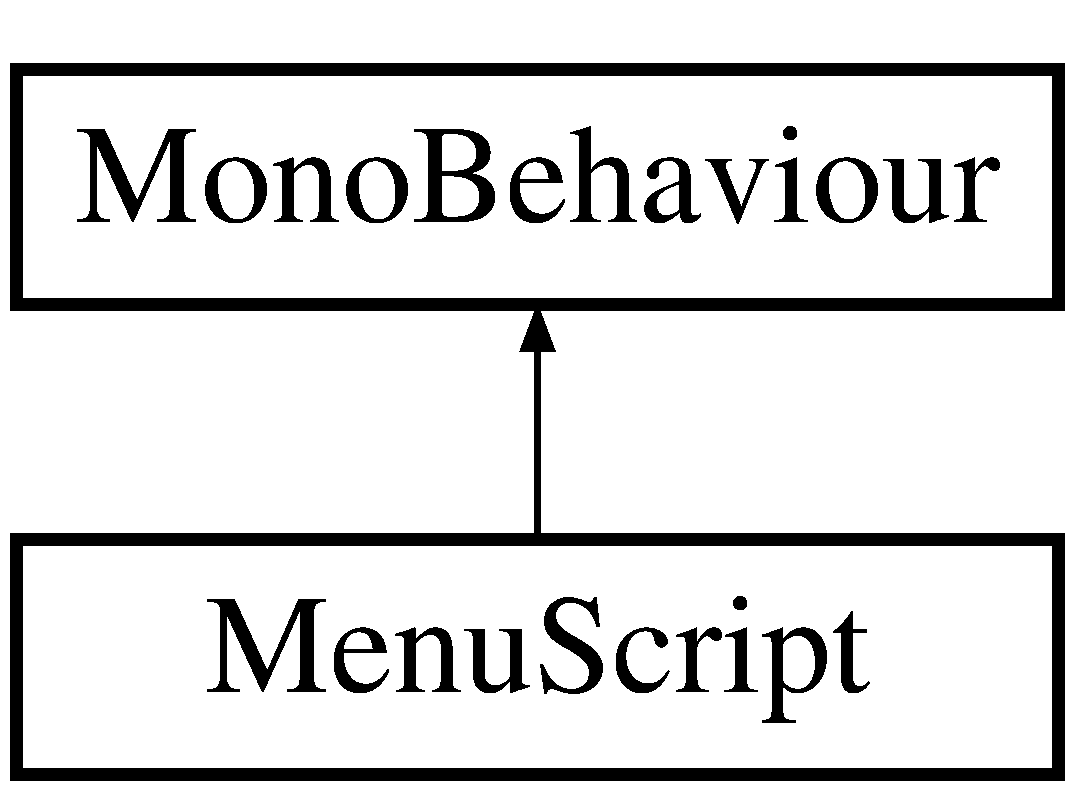
\includegraphics[height=2.000000cm]{class_menu_script}
\end{center}
\end{figure}
\subsection*{Public Types}
\begin{DoxyCompactItemize}
\item 
\mbox{\Hypertarget{class_menu_script_abcfacec71044638c8ccc3b6e04cc39f8}\label{class_menu_script_abcfacec71044638c8ccc3b6e04cc39f8}} 
enum {\bfseries \+\_\+\+Menu} \{ {\bfseries P\+L\+AY}, 
{\bfseries E\+X\+IT}, 
{\bfseries A\+B\+O\+UT}, 
{\bfseries S\+T\+A\+R\+T\+I\+N\+G\+A\+ME}
 \}
\end{DoxyCompactItemize}
\subsection*{Public Member Functions}
\begin{DoxyCompactItemize}
\item 
\mbox{\Hypertarget{class_menu_script_a7fd4869b3bcf92a8a71a2bcbb7758770}\label{class_menu_script_a7fd4869b3bcf92a8a71a2bcbb7758770}} 
void {\bfseries Update\+Menu} (Image image, Sprite sprite)
\item 
\mbox{\Hypertarget{class_menu_script_a7e50d38073f9796c3035ab0b5a562003}\label{class_menu_script_a7e50d38073f9796c3035ab0b5a562003}} 
void {\bfseries Start} ()
\item 
\mbox{\Hypertarget{class_menu_script_ab87c9e111bf4e379a062c7d135551534}\label{class_menu_script_ab87c9e111bf4e379a062c7d135551534}} 
void {\bfseries Info} ()
\item 
\mbox{\Hypertarget{class_menu_script_a140002b1c2186b0223d79dddccb602fd}\label{class_menu_script_a140002b1c2186b0223d79dddccb602fd}} 
void {\bfseries Exit} ()
\item 
\mbox{\Hypertarget{class_menu_script_a672eb8f935132634bc958abba0804373}\label{class_menu_script_a672eb8f935132634bc958abba0804373}} 
void {\bfseries Text\+Control} (bool sobre, bool saida)
\item 
\mbox{\Hypertarget{class_menu_script_a3ff96c7af5b82f1b2bb09b02ea8a7511}\label{class_menu_script_a3ff96c7af5b82f1b2bb09b02ea8a7511}} 
void {\bfseries Exit\+Game} ()
\item 
\mbox{\Hypertarget{class_menu_script_a9347d5e7759ebceb5b1266faca8d336b}\label{class_menu_script_a9347d5e7759ebceb5b1266faca8d336b}} 
void {\bfseries Start\+Game} ()
\item 
\mbox{\Hypertarget{class_menu_script_a59a03a9700356cfe75901d841a7fda97}\label{class_menu_script_a59a03a9700356cfe75901d841a7fda97}} 
void {\bfseries Starting} ()
\end{DoxyCompactItemize}
\subsection*{Public Attributes}
\begin{DoxyCompactItemize}
\item 
\mbox{\Hypertarget{class_menu_script_a0f0bd96677862565dd499cfc5a3c02b1}\label{class_menu_script_a0f0bd96677862565dd499cfc5a3c02b1}} 
Image {\bfseries \+\_\+\+Main\+Image}
\item 
\mbox{\Hypertarget{class_menu_script_ad2811488825fef6ae54499488cf704b2}\label{class_menu_script_ad2811488825fef6ae54499488cf704b2}} 
Image {\bfseries \+\_\+container}
\item 
\mbox{\Hypertarget{class_menu_script_ab6a92190bfed825f9ad41d849fc5a1b3}\label{class_menu_script_ab6a92190bfed825f9ad41d849fc5a1b3}} 
Sprite {\bfseries \+\_\+\+Play\+Selected}
\item 
\mbox{\Hypertarget{class_menu_script_a2e78e58cb803592e5c2399b0f50ad1e1}\label{class_menu_script_a2e78e58cb803592e5c2399b0f50ad1e1}} 
Sprite {\bfseries \+\_\+\+Info\+Selected}
\item 
\mbox{\Hypertarget{class_menu_script_a385622f8e918dff3ac1d7b5319cdde32}\label{class_menu_script_a385622f8e918dff3ac1d7b5319cdde32}} 
Sprite {\bfseries \+\_\+\+Exit\+Selected}
\item 
\mbox{\Hypertarget{class_menu_script_aaee8ba76cf4cdf118d19d6e2874924d4}\label{class_menu_script_aaee8ba76cf4cdf118d19d6e2874924d4}} 
Sprite {\bfseries \+\_\+\+Title\+On}
\item 
\mbox{\Hypertarget{class_menu_script_a60287f8918307e1066a5188c80eadb24}\label{class_menu_script_a60287f8918307e1066a5188c80eadb24}} 
Sprite {\bfseries \+\_\+about\+On}
\item 
\mbox{\Hypertarget{class_menu_script_a060fdf985ea3a748ab76b66cc282b2d4}\label{class_menu_script_a060fdf985ea3a748ab76b66cc282b2d4}} 
\+\_\+\+Menu {\bfseries \+\_\+menu}
\item 
\mbox{\Hypertarget{class_menu_script_a55ac367e2c7fa495a9dfb038cb256bb5}\label{class_menu_script_a55ac367e2c7fa495a9dfb038cb256bb5}} 
Text {\bfseries \+\_\+about\+Text}
\item 
\mbox{\Hypertarget{class_menu_script_ad97f41b371f89a89c3bf9190e50e50d9}\label{class_menu_script_ad97f41b371f89a89c3bf9190e50e50d9}} 
Text {\bfseries \+\_\+\+Exit\+Text}
\item 
\mbox{\Hypertarget{class_menu_script_a7256fc432e031026ad6302e5fe6f7bd7}\label{class_menu_script_a7256fc432e031026ad6302e5fe6f7bd7}} 
bool {\bfseries \+\_\+\+One\+Click}
\item 
\mbox{\Hypertarget{class_menu_script_ad28acc9f1c2aeecd423e49955a5ffae0}\label{class_menu_script_ad28acc9f1c2aeecd423e49955a5ffae0}} 
string {\bfseries \+\_\+\+Prox\+Cena}
\item 
\mbox{\Hypertarget{class_menu_script_a2571fdf4c2f039b286c4bd5e0f608b21}\label{class_menu_script_a2571fdf4c2f039b286c4bd5e0f608b21}} 
Image {\bfseries \+\_\+next}
\item 
\mbox{\Hypertarget{class_menu_script_a7ecadb07a98acdeeb7edb34d6b7a1fe7}\label{class_menu_script_a7ecadb07a98acdeeb7edb34d6b7a1fe7}} 
Button \mbox{[}$\,$\mbox{]} {\bfseries \+\_\+buttons}
\end{DoxyCompactItemize}


The documentation for this class was generated from the following file\+:\begin{DoxyCompactItemize}
\item 
Menu\+Script.\+cs\end{DoxyCompactItemize}

\hypertarget{struct_pallete}{}\section{Pallete Struct Reference}
\label{struct_pallete}\index{Pallete@{Pallete}}
\subsection*{Public Attributes}
\begin{DoxyCompactItemize}
\item 
\mbox{\Hypertarget{struct_pallete_a3ea2b6f82cfdb219a82bdf5239fd9f08}\label{struct_pallete_a3ea2b6f82cfdb219a82bdf5239fd9f08}} 
Color \mbox{[}$\,$\mbox{]} {\bfseries color\+Pallete}
\end{DoxyCompactItemize}


The documentation for this struct was generated from the following file\+:\begin{DoxyCompactItemize}
\item 
Color\+Pallete.\+cs\end{DoxyCompactItemize}

\hypertarget{class_random_color}{}\section{Random\+Color Class Reference}
\label{class_random_color}\index{Random\+Color@{Random\+Color}}
Inheritance diagram for Random\+Color\+:\begin{figure}[H]
\begin{center}
\leavevmode
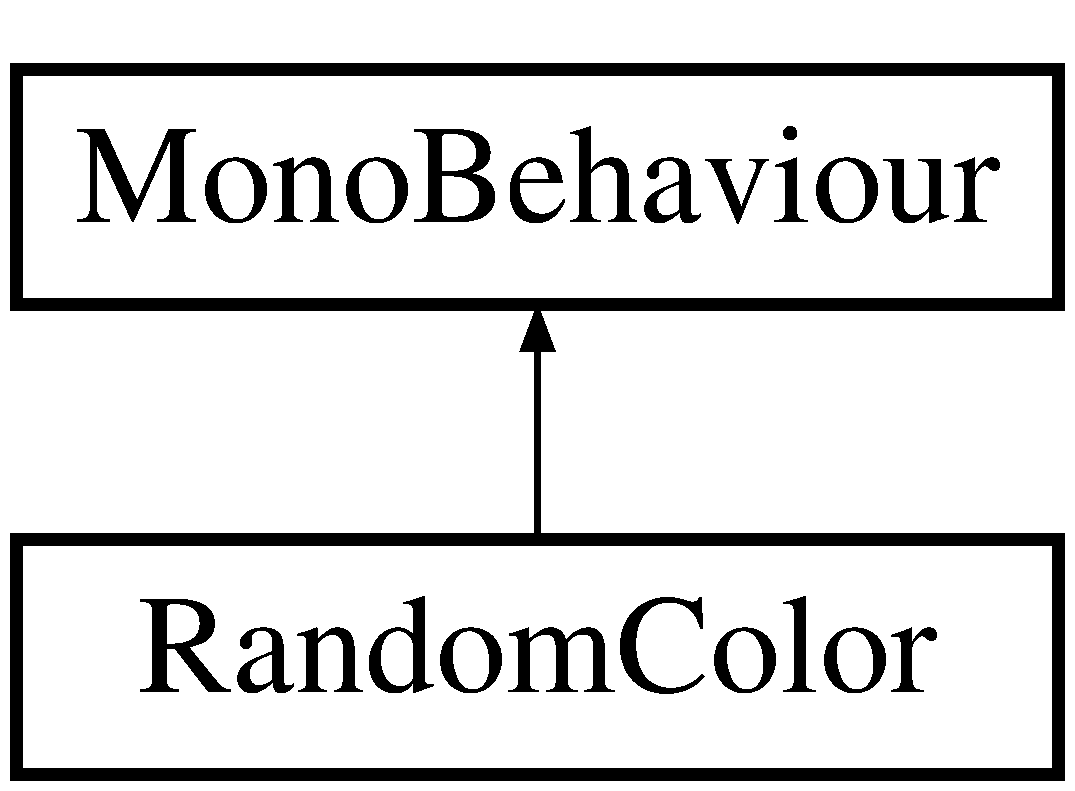
\includegraphics[height=2.000000cm]{class_random_color}
\end{center}
\end{figure}
\subsection*{Public Attributes}
\begin{DoxyCompactItemize}
\item 
\mbox{\Hypertarget{class_random_color_ad6618129e199ffac1319e1f7658e292b}\label{class_random_color_ad6618129e199ffac1319e1f7658e292b}} 
Color \mbox{[}$\,$\mbox{]} {\bfseries \+\_\+cores\+In\+Game}
\end{DoxyCompactItemize}


The documentation for this class was generated from the following file\+:\begin{DoxyCompactItemize}
\item 
Random\+Color.\+cs\end{DoxyCompactItemize}

\hypertarget{class_tutorial_script}{}\section{Tutorial\+Script Class Reference}
\label{class_tutorial_script}\index{Tutorial\+Script@{Tutorial\+Script}}
Inheritance diagram for Tutorial\+Script\+:\begin{figure}[H]
\begin{center}
\leavevmode
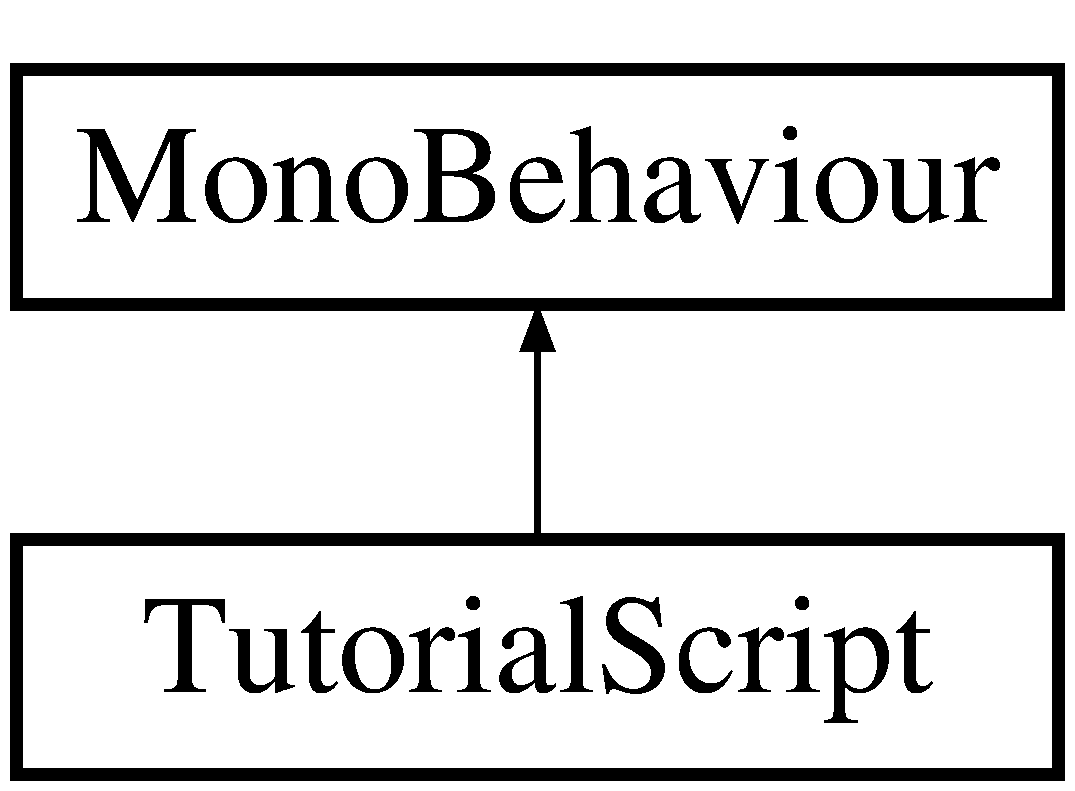
\includegraphics[height=2.000000cm]{class_tutorial_script}
\end{center}
\end{figure}
\subsection*{Public Types}
\begin{DoxyCompactItemize}
\item 
\mbox{\Hypertarget{class_tutorial_script_a4df778a9d233c279e7b66bd97b634a9b}\label{class_tutorial_script_a4df778a9d233c279e7b66bd97b634a9b}} 
enum {\bfseries \+\_\+\+T\+U\+T\+O\+R\+I\+AL} \{ {\bfseries W\+E\+L\+C\+O\+ME}, 
{\bfseries P\+L\+A\+Y\+I\+NG}, 
{\bfseries G\+A\+M\+E\+O\+V\+ER}
 \}
\end{DoxyCompactItemize}
\subsection*{Public Attributes}
\begin{DoxyCompactItemize}
\item 
\mbox{\Hypertarget{class_tutorial_script_ab52722849cff3356825d7b90fa65a283}\label{class_tutorial_script_ab52722849cff3356825d7b90fa65a283}} 
Game\+Object {\bfseries \+\_\+\+Tutorial\+H\+UD}
\item 
\mbox{\Hypertarget{class_tutorial_script_a376788b5e6e5696201a63d56282018d3}\label{class_tutorial_script_a376788b5e6e5696201a63d56282018d3}} 
Game\+Object {\bfseries \+\_\+\+Game\+H\+UD}
\item 
\mbox{\Hypertarget{class_tutorial_script_a22a7be7d7dade111770af91fc14a4fcf}\label{class_tutorial_script_a22a7be7d7dade111770af91fc14a4fcf}} 
\+\_\+\+T\+U\+T\+O\+R\+I\+AL {\bfseries \+\_\+tutorial}
\item 
\mbox{\Hypertarget{class_tutorial_script_a9d830927189e92f9be029a5ad164ce67}\label{class_tutorial_script_a9d830927189e92f9be029a5ad164ce67}} 
Sprite \mbox{[}$\,$\mbox{]} {\bfseries \+\_\+tuto\+Text}
\item 
\mbox{\Hypertarget{class_tutorial_script_a025ae0fa91ceaa15d99bf7130ea423ee}\label{class_tutorial_script_a025ae0fa91ceaa15d99bf7130ea423ee}} 
Image {\bfseries \+\_\+tuto\+Box}
\item 
\mbox{\Hypertarget{class_tutorial_script_af4d0216904eb3e7b6ac825cb93bb7bf3}\label{class_tutorial_script_af4d0216904eb3e7b6ac825cb93bb7bf3}} 
Image {\bfseries \+\_\+tuto\+Info}
\item 
\mbox{\Hypertarget{class_tutorial_script_a7e4070a38c83a4c7b6091c06a2a20be8}\label{class_tutorial_script_a7e4070a38c83a4c7b6091c06a2a20be8}} 
Sprite\+Renderer {\bfseries \+\_\+loading}
\end{DoxyCompactItemize}


The documentation for this class was generated from the following file\+:\begin{DoxyCompactItemize}
\item 
Tutorial\+Script.\+cs\end{DoxyCompactItemize}

%--- End generated contents ---

% Index
\backmatter
\newpage
\phantomsection
\clearemptydoublepage
\addcontentsline{toc}{chapter}{Index}
\printindex

\end{document}
